% !TeX spellcheck = sv_SE
% !TeX encoding = UTF-8
%%%%%%%%%%%%%%%%%%%%%%%%%%%%%%%%%%%%%%%%%%%%%%%%%%%%%%%%%%%%%%%%%%%%%%%%%%%%%%
% Krisradiomall
%
% Mall i LaTeX av Täpp-Anders Sikvall
% 2019-03-11 anders@sikvall.se
%
% Får användas utan medgivande så länge som denna kommentar
% finns kvar i filen. Ändringar är förstås tillåtna i övrigt
%
%%%%%%%%%%%%%%%%%%%%%%%%%%%%%%%%%%%%%%%%%%%%%%%%%%%%%%%%%%%%%%%%%%%%%%%%%%%%%%
\documentclass[a4paper,10pt]{article}
\usepackage[a4paper]{geometry}
\usepackage[english]{babel}
\usepackage{soul}
\usepackage{graphicx}
\usepackage[table,x11names]{xcolor}
\usepackage{atbegshi}
\usepackage{fancyhdr}
\usepackage{amsmath}
\usepackage{MnSymbol}
\usepackage{wasysym}
\usepackage{lipsum}
\usepackage{tabularx}
\usepackage[yyyymmdd]{datetime} \renewcommand{\dateseparator}{-}
\usepackage[utf8]{inputenc}
\usepackage{lastpage}
\usepackage[scaled]{helvet} 	\renewcommand\familydefault{\sfdefault} 
\usepackage[italic]{mathastext}
\usepackage{isomath}
\usepackage[T1]{fontenc}
\usepackage[hidelinks]{hyperref}
\usepackage{enumitem}
\usepackage{marginnote}
\usepackage{pdfpages}
\usepackage{icomma}
\usepackage{pdflscape}
\usepackage{wrapfig}
\usepackage{float}
\usepackage[bottom]{footmisc}
\usepackage{longtable}
\usepackage{gensymb}
\usepackage{tikz}
\usetikzlibrary{arrows,chains,positioning,patterns,calc}
\newif\iftitlefoot
\raggedbottom
\usepackage{enumitem}
\setlist{nosep}
\usepackage{todonotes}
%\usepackage{draftwatermark}
%\SetWatermarkText{GRANSKAS}
%\SetWatermarkScale{.7}
%\SetWatermarkLightness{.7}

%%%%%%%%%%%%%%%%%%%%%%%%%%%%%%%%%%%%%%%%%%%%%%%%%%%%%%%%%%%%%%
%%%%% Definiera diverse saker här som används i dokumentet
\newcommand{\TitleText}{KRISRADIOHANDBOKEN}
\newcommand{\SubtitleText}{Privatradio och Amatörradio}
\newcommand{\Forfattare}{Anders Sikvall}
\newcommand{\Initialer}{ANSI}
\newcommand{\DokYear}{2019}
\newcommand{\DokNr}{-03}
\newcommand{\DokumentRevision}{A}

\newcommand{\Mottagare}{Allmänt publicerad}
\newcommand{\DokumentDatum}{\today}
\newcommand{\DokumentNummer}{\Initialer -\DokYear :\DokNr/\DokumentRevision}
%%%%%%%%%%%%%%%%%%%%%%%%%%%%%%%%%%%%%%%%%%%%%%%%%%%%%%%%%%%%%%%%%%




%\titlefootfalse % Använd denna för ren förstasida
\titlefoottrue % Använd denna för en footer på första sidan
\newcommand{\titlefootcontent}{%
	\begin{tabularx}{.9\textwidth}{X X X X}	%
		\textbf{Mottagare} & \textbf{Författare} & \textbf{Datum}  & \textbf{Dok. Nr.} \\		%
		\Mottagare       & \Forfattare          & \DokumentDatum & \DokumentNummer   \\		%            
	\end{tabularx}%
}

\addtolength{\headsep}{-3mm}
\addtolength{\textheight}{15mm}

\begin{document}


%%%%%%%%%%%%%%%%%%%%%%%%%%%%%%%%%%%
%%% Bygger förstasidan här

\newgeometry{left=2cm,right=2cm,bottom=1cm,top=1cm}
\pagestyle{empty}
\vfill
\begin{flushright}
	
\includegraphics[width=0.25\textwidth]{Logo/krh-logo}
\end{flushright}
\vspace*{4cm}
\centerline{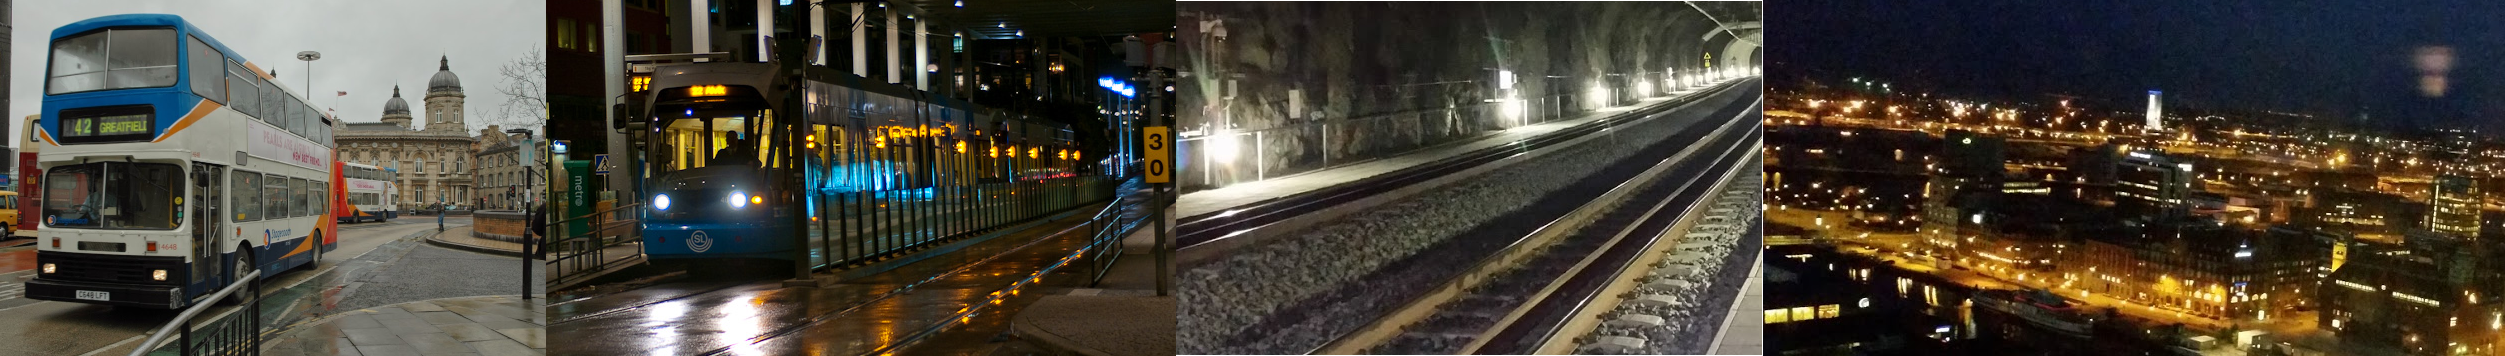
\includegraphics[width=\paperwidth]{Logo/krh-rubrikbild}}
\begin{flushright}
	\Huge{\bfseries{\TitleText}} \\[3mm]
	\Large{\bfseries{\SubtitleText}}
\end{flushright}

\vfill
	
\small
\begin{tabular}{llll}
	\textbf{Rev} & \textbf{Date} & \textbf{Responsible} & \textbf{Description} \\ \hline
	A            & \today         & ANSI              & Pågående revision
\end{tabular}
\normalsize 
\vfill

\iftitlefoot
\scriptsize
\vspace*{-1em}
\hrule
\begin{center}
	\begin{tabularx}{.9\textwidth}{X X X X}
		\titlefootcontent &
\end{tabularx}
\end{center}
\normalsize
\fi
\newpage

%\restoregeometry

\newgeometry{top=3cm}

\pagestyle{fancy}
%\setlength{\headheight}{53pt} 

\lhead{
\includegraphics[height=10pt]{Logo/krh-logo}}

\rhead{
	\scriptsize
	\begin{tabular}{lll}
		\textbf{Date} & \textbf{DocNr} & \textbf{Rev.}\\
		\DokumentDatum & \DokumentNummer & \DokumentRevision \\
	\end{tabular}
}

\chead{}

\lfoot{
	\scriptsize
	Täpp-Anders Sikvall\\
	anders@sikvall.se
}

\cfoot{\scriptsize \thepage\ / \pageref{LastPage}}

\rfoot{
	\scriptsize
	www.krisradio.se\\
	Twitter: ichimusaiSWE
}

\renewcommand{\footrulewidth}{0.2pt}

\widowpenalty=9999
\clubpenalty=9999

%	\setlength{\headsep}{1em}2


%%%%%%%%%%%%%%%%%%%%%%%%%%%%%%%%%%%%%%%%%%%%%%%%%%%%%
%%% Här börjar dokumentet som skall redigeras
%

\cleardoublepage
%\newgeometry{left=3.2cm,right=3.2cm,bottom=2.5cm,top=2.5cm}

%%% Innehållsförteckning
\tableofcontents

\newpage

% Lista bilagor här

%\listoffigures

%\listoftables

%\listoftodos


%%% Justera här om du föredrar indrag som i löpande text. Teknisk dokumentation
%%% tycker jag fungerar bättre med styckenmellanrum utan indrag. \parskip justerar
%%% styckemellanrum och \parindent är indrag.
\setlength{\parskip}  {1ex}
\setlength{\parindent}{0pt}

%%% Dokumentets egentliga innehåll

\section{Inledning}

\subsection{Privatradio och Amatörradio}

\subsection{Med enkla medel}



\section{Innan krisen kommer}

\subsection{Förberedelser innan krisen}

\subsection{Samövning och samordning}

\subsection{Lär barnen}

\section{Om krisen kommer}

\subsection{Att få kontakt}

\subsubsection{Samband inom familjen}

\subsubsection{Nå grannarna}

\subsubsection{På längre avstånd}





\section{Din anläggning}

\subsection{Utrustning}

\subsection{Antenner}



\section{Teknisk information}

\subsection{Frekvenser}

\subsection{Signalstyrka}


\end{document}
